%# -*- coding: utf-8-unix -*-
%%==================================================
%% 03_zuc.tex % 2.5k
%%==================================================

\chapter{ZUC 算法的软硬件实现以及攻击方案}

\label{chap:zuc}

\section{算法背景} % 0.5k
% 《3GPP LTE 国际加密标准 ZUC 算法》
祖冲之算法,又称 ZUC 算法,是我国提出的第一个国际商用标准密码算法。

2004 年,3GPP(3rd Generation Partnership Project,第三代合作伙伴计划)提出了 LTE(Long Term Evolution,长期演进),目的是保证该计划能够继续在电信行业拥有一定的话语权。在 2010 年底,3GPP 被确立为第四代(4G)移动通信标准。 \cite{lte}

安全性是通信技术中一个非常重要的指标,而密码算法又是保障安全性的一个重要工具。3GPP 之前已经拥有的两个算法是 AES 和 SNOW 3G,而 ZUC 算法则是第三个被纳入标准的算法。ZUC 算法的提出和设计历经了很多挑战,因为商用密码算法的要求非常严苛,既要保证极高的安全性,又要拥有较高地运行性能,还需要在各自环境下都方便实现。中国科学院等单位克服了重重困难,最终研制成功,经由中国通信标准化协会与工信部向 3GPP 组织提交了这一算法,并且经过了行业严格的评审,最终被批准成为 LTE 中的密码算法标准,参与到实际的商业应用。 \cite{zuc_test}

总之,ZUC 算法的提出,使我国在国际商用密码领域拥有了更多的自主权,既体现了我国在密码学领域的学术能力,又是我国参与制定国际化通信标准的重要一步。因此,研究 ZUC 算法,具有很高的现实意义。

\section{算法流程} % 1k

ZUC 算法分成三层,如下: \cite{zuc_standard}

\begin{itemize}
    \item \textbf{线性反馈移位寄存器(Linear feedback shift register,LFSR):}LFSR 有两种模式,初始化模式和工作模式。
    \item \textbf{比特重组(Bit Reorgnization, BR):}该层将寄存器中特定位置的数据进行编排然后输出。
    \item \textbf{非线性函数(Nonlinear Function, F):}这一层涉及到一个 S 盒置换,而 S 盒置换是非线性的,因此也是这个算法中非常关键的部分。我们后续的功耗分析攻击,将会重点关注这一部分。
\end{itemize}

\vspace*{\baselineskip}

ZUC 算法的运行过程如下:\cite{zuc_standard}

\begin{enumerate}
    \item \textbf{初始化阶段:}这一部分包括初始密钥的装载,LFSR 和寄存器的初始化,以及重复 32 轮的打乱操作(每一轮都包含比特重组、非线性函数以及以初始模式运行一次 LFSR)。
    \item \textbf{工作阶段:}这一部分包括一个一次性操作(比特重组、非线性函数以及以工作模式运行一次 LFSR)以及密钥生成阶段(每一次密钥输出都包含比特重组、非线性函数、输出密钥以及以工作模式运行一次 LFSR)。
\end{enumerate}

\vspace*{\baselineskip}

由于密码本身相对比较复杂,尽管我已经在硬件和软件上都实现 ZUC 算法,并且验证了实现的正确性,然而想要解释清楚一些实现中具体的细节,还是太过冗长了,而且毫无必要,因此这里只是粗略地介绍了一下算法的基本组成部分和大致流程。如果想要了解关于算法的更多信息,可以参考文献 \parencite{zuc_standard}。

作为攻击者和研究人员,了解算法的全部细节和设计理由固然重要,但是更加重要的是找到算法在实际实现中可能存在的问题。设计者和攻击者考虑问题的角度是不一样的,设计者往往拥有更好的大局观,但在细节上往往无法挖掘太深,而攻击者只需要撬动整个系统中的某一点就足以达成目标了。

因此我们将在下一小节讨论对 ZUC 算法实施差分功耗攻击的方法。

\vspace*{\baselineskip}

图 \ref{fig:zuc_algo} 展示了 ZUC 算法的过程。

\begin{figure}[htbp]
    \centering
    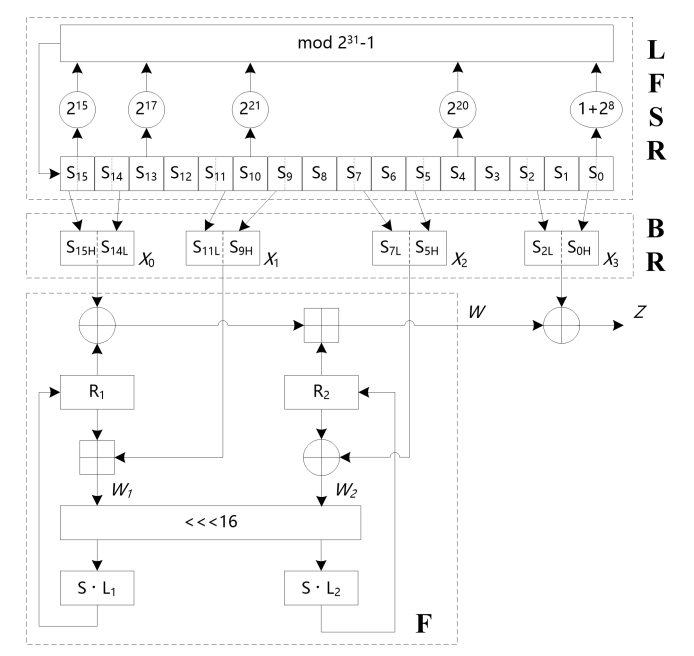
\includegraphics[height=.5\textheight]{../images/zuc_algo.png}
    \caption{ZUC 算法的流程图 \cite{zuc_standard}}
    \label{fig:zuc_algo}
\end{figure}


\section{算法的软硬件实现}

硬件设计使用的软件是 ISE 14.3,使用的 FPGA 型号为:XC6SLX75-2CSG484。在完成硬件设计、仿真和综合后,在实际环境中运行 ZUC 算法,并采集功耗曲线,用于后续的分析

软件实现使用的语言为 Python 3.6,运行平台为 Windows 10。软件部分的作用是在功耗分析过程中计算中间值以及对应的假设功耗值,并进行相关系数攻击和更多的处理。软件代码开源在本人的 GitHub 仓库中:https://github.com/Hansimov/zuc-attack。

\newpage

硬件电路的输入和输出端口如图 \ref{fig:circuit_io} 所示。

\begin{figure}[htbp]
    \centering
    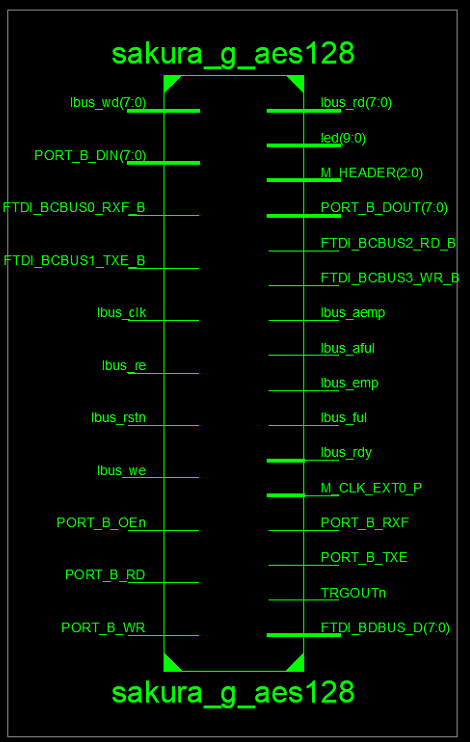
\includegraphics[height=.6\textheight]{../images/circuit_io.png}
    \caption{硬件电路的输入和输出端口}
    \label{fig:circuit_io}
\end{figure}

\newpage

硬件电路的内部结构如图 \ref{fig:circuit_more} 所示。

\begin{figure}[htbp]
    \centering
    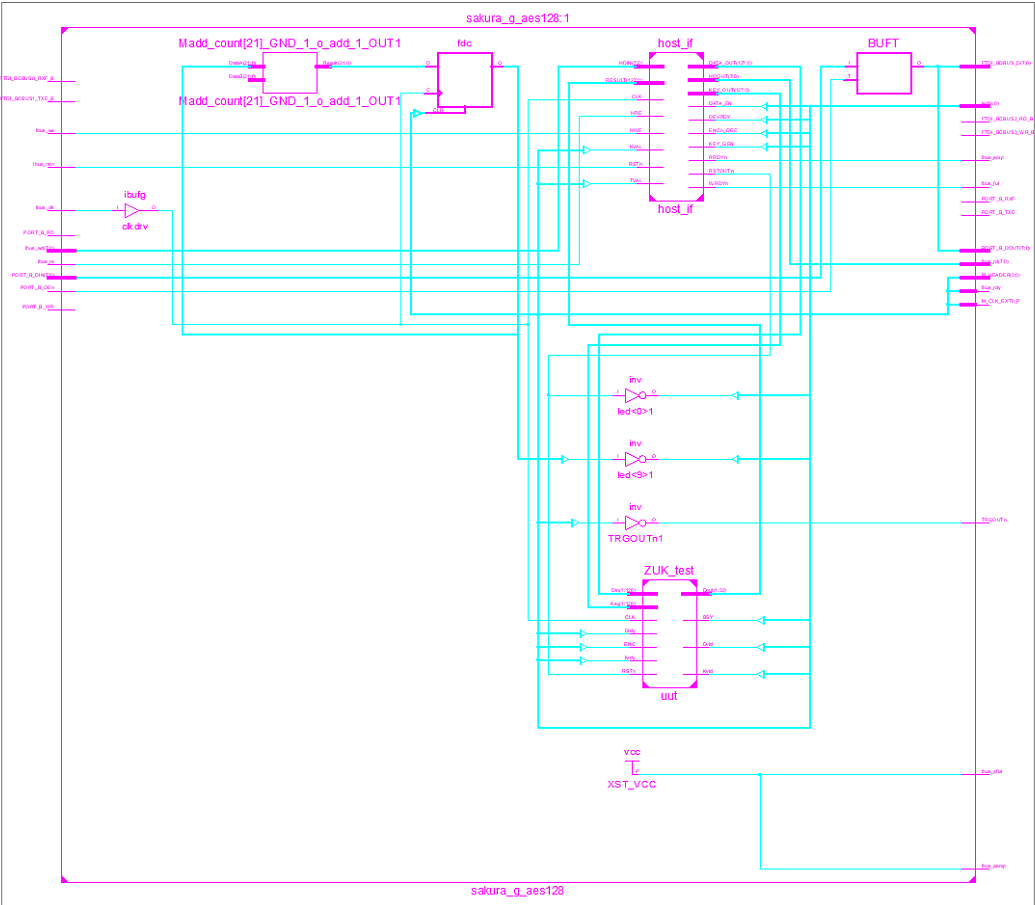
\includegraphics[height=.6\textheight]{../images/circuit_more.png}
    \caption{硬件电路的内部结构}
    \label{fig:circuit_more}
\end{figure}

\newpage

\section{对 ZUC 算法的差分功耗分析方案} % 1k
\label{sec:zuc_attack}

小节 \ref{sec:dpa} 阐述了差分功耗攻击的基本方法,而本小节将把这个方法应用到具体的算法上。

在 ZUC 算法中,唯一未知的信息就是初始密钥,其他的常量和明文都是已知的。因此我们的攻击目的就是得到密钥的信息。

差分功耗攻击最核心的思想是,假设功耗值和实际功耗值之间是有关联的。而要想假设功耗值尽可能贴合实际功耗值,就需要选择合适的中间值,采用合适的功耗模型。一般而言,中间值通常选择算法中非线性变换的部分,因为如果输入稍有不同,非线性变换的输出就会出现较大的差异,因此,正确的输入和错误的输入产生的差异将比线性变换更加明显,就可以有效地区分出正确的输入和错误的输入。功耗模型通常选择汉明重量模型或者比特模型,为了方便,我们这里采用汉明重量模型。

\vspace*{\baselineskip}

差分功耗分析的第一步是要在硬件上实现 ZUC 算法电路,然后采集其运行时的功耗。这部分和针对其他算法的差分功耗分析没有什么差别,因此不再详细说明。我们重点关注分析 ZUC 算法中的特别之处。

\vspace*{\baselineskip}

图 \ref{fig:zuc_attack} 展示了 ZUC 算法中可以利用的漏洞。在 ZUC 算法初始化阶段的第一轮打乱操作中,非线性函数中左侧寄存器的输出仅和 k9 这个密钥字节相关,右侧寄存器的输出仅和 k5 这个密钥字节相关。 \cite{zuc_attack_tangming}

\begin{figure}[htbp]
    \centering
    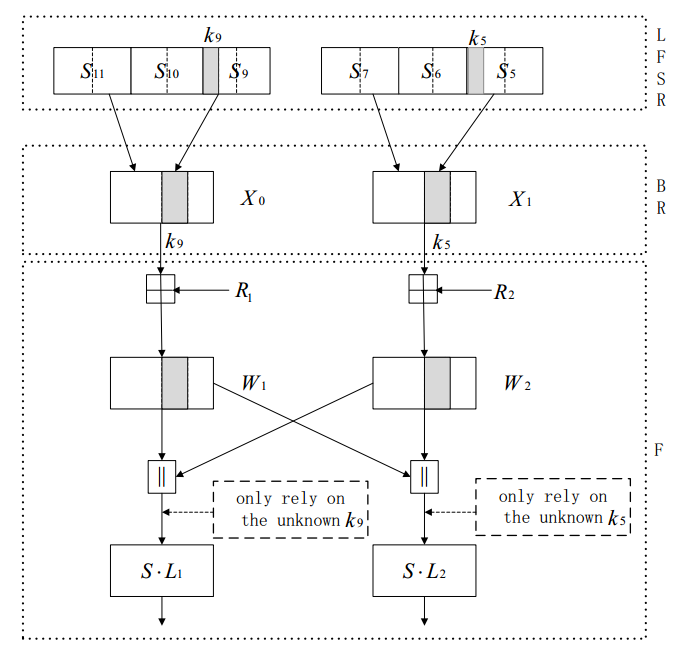
\includegraphics[height=.5\textheight]{../images/zuc_attack.png}
    \caption{非线性函数中左侧寄存器的输出仅和 k9 相关,右侧寄存器的输出仅和 k5 相关\cite{zuc_attack_tangming}}
    \label{fig:zuc_attack}

\end{figure}

因此,选择初始化阶段第一轮打乱操作中,非线性函数右半部分的输出作为我们的中间值,尝试攻击出 k5 的值。

\vspace*{\baselineskip}

选择这个位置作为中间值有两个原因:

\begin{enumerate}
    \item \textbf{这个位置仅仅和单个密钥字节(k5)相关,和其他的密钥字节没有任何关系。}这意味着我们只需要猜测 $2^8=256$ 中情况,大大减少了工作量。如果选择某个其他的中间值,很可能和多个密钥字节有关联,我们假设关联的密钥字节数为 N,那么我们就需要猜测 $2^{8 \times N}$ 中情况。可以想象,如果关联的密钥字节很多的话,我们需要猜测的可能情况就会爆炸式增长,由于我们只拥有有限的计算资源,因此这是不能接受的。
    \item \textbf{这个位置是非线性变换(S 盒置换)的输出,因而正确猜测和错误猜测之间的差异较为明显。}这一点我们在上面已经提及,因此不再赘述。
\end{enumerate}

\vspace*{\baselineskip}

选择好了中间值,我们就可以通过编程计算出所有密钥猜测(从 0 到 255,也即 16 进制的 00 到 FF)对应的的中间值。

有了中间值之后,我们就可以根据汉明重量模型,计算出理论功耗值(也就是假设功耗值)。然后我们实施相关系数攻击,也即计算假设功耗值和实际功耗值之间的相关系数(在本次实验中,这个值还需要稍微处理一下,得到更加可靠的相对相关系数),然后分析相对相关系数,值最大的即对应最优的密钥猜测。

这就是对 ZUC 算法进行功耗分析攻击的大致流程,我们将在下一小节展示相关的实验结果,并补充一些实现细节。

\section{本章小结}

本章首先讨论了 ZUC 算法的提出背景,介绍了其和通信行业发展的密切联系,并且指出了该算法对我国的重要意义。

然后我们讨论了 ZUC 算法的流程和结构,分别介绍了 ZUC 算法的三个部分,包括线性移位反馈寄存器、比特重组和非线性函数,并且讲解了初始化和工作的运行过程。

接着我们展示了 ZUC 算法的软硬件实现情况,给出了硬件电路的原理图,开源了软件代码,并且介绍了硬件部分和软件部分各自的用途。

最后我们讨论了针对 ZUC 算法的差分功耗分析方案,除了介绍了传统的差分功耗分析的流程,还依据相关资料选取了有效的中间值,并且解释了这样选取的具体原因。
